\documentclass[11pt,a4paper]{article} 

\usepackage[dutch]{babel} %needs to specified for minutes package (else it will be in German)
\usepackage{a4wide}%For a wider spacing of the text (smaller left/right margin)
\usepackage{graphicx}
\usepackage{setspace}
\usepackage{minutes}

\pagestyle{plain}
\usepackage{todositemized}
%more memmorable commands to make the checked and crossed symbols





%%%%%%%%%%%%%%%%%%%%%%%%%%%%%%%%%%%%%%%%%%%%%%%%%%%%%%%%%%%%%%%%%%%%%%%%%%%%%%%
%
% Important: This template compiles without errors
% always check errors, also the yellow ones, even if you get a PDF
%
%%%%%%%%%%%%%%%%%%%%%%%%%%%%%%%%%%%%%%%%%%%%%%%%%%%%%%%%%%%%%%%%%%%%%%%%%%%%%%%%





\newpage



\usepackage[dutch]{babel} %needs to specified for minutes package (else it will be in German)
\usepackage{a4wide}%For a wider spacing of the text (smaller left/right margin)

\usepackage{setspace}
\usepackage{minutes}

\pagestyle{plain}
\usepackage{todositemized}
%more memmorable commands to make the checked and crossed symbols





%%%%%%%%%%%%%%%%%%%%%%%%%%%%%%%%%%%%%%%%%%%%%%%%%%%%%%%%%%%%%%%%%%%%%%%%%%%%%%%
%
% Important: This template compiles without errors
% always check errors, also the yellow ones, even if you get a PDF
%
%%%%%%%%%%%%%%%%%%%%%%%%%%%%%%%%%%%%%%%%%%%%%%%%%%%%%%%%%%%%%%%%%%%%%%%%%%%%%%%%



\begin{document}

\begin{Minutes}{Notulen Poject Natuurkunde, groepje 24}


%Add relevant date, time and location here
\minutesdate{12-06-2023} %Write the date of when you finish the minutes
\starttime{11:00}
\endtime{}
\location{}

%Add relevant names here
\participant{Tom, Noah} 
\minutetaker{Tom}

% \moderation{Niemand} 
%In case people are not present


\maketitle



\newpage


\section{Mededelingen} 
Vandaag begonnen we om 11 uur, de dag startte met Noah die verder was gegaan met het programmeren met zijn code van gister om de metingen te plaatsen op een grafiek met als y-as eta en als x-as omega. Antione heeft Tom bijgepraat omdat hij op 11 juni ziek was. Daarna hebben we de viscositeit van de beige putty opnieuw gemeten. Aan het eind van de dag heeft Noah gewerkt om een fit te maken voor $E^*$ en een factor $\alpha$ en heeft Tom gewerkt aan de geshifte data te overlappen met de data op 20 graden. Om 5 uur zijn we naar huis gegaan. Verder waren Madelief en Talha absent, Madelief is gestopt met het project en Talha had een stagedag op een middelbare school.

\section{Experiment}
Het meten van de viscositeit van de beige putty is gedaan met de reometer. We hadden al een keer beige putty met dit apparaat gemeten maar het bereik was niet groot genoeg, door gebruik te maken van de time-temperature superposition konden we het bereik vergroten, maar dan moest een plaat naar -15 graden celsius gekoeld worden. Echter het probleem was dat het water in de lucht op de plaat bevroor waardoor de meting niet exact genoeg uitgevoerd kon worden, we hebben dit eerst proberen op te lossen door schuurpapier aan de plaat vast te maken zodat de klei genoeg adhesie had aan de plaat maar dat er op het schuurpapier hopelijk geen ijs kwam. Dit was echter nog steeds het geval, daarna hebben we gebruikgemaakt van een plastic kast die we om de reometer hebben heengezet en daarna gevuld met stikstof zodat er geen waterstof meer in de lucht zat. Dit werkte wel goed. 


\section{Wat moeten we nu doen/bespreken?}
We willen morgen (13 juni) de videometingen helemaal afhebben door de soft en medium putty te omhulsen met magnesiumpoeder zodat er geen adhesie meer is. Ook willen we op min 30 graden (of ergens in de trant) de viscositeit meten zodat we het hele bereik van de elastische eigenschappen van de putty kunnen krijgen.

\section{Figuren}
\begin{figure}[h]
    \centering
    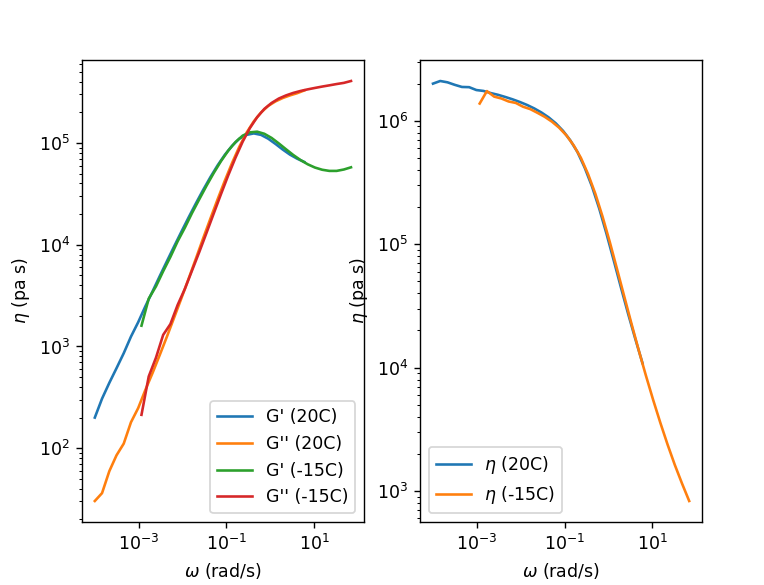
\includegraphics[width=0.5\linewidth]{Rheometerdata.png}
    \caption{In de linker grafiek is de data te zien van G' en G'', die het gedrag van de putty als vloeistof of als elastische stof beschrijft. Deze zijn overlapt over elkaar door de grafiek van -15 graden met een factor te vermenigvuldigen, In de rechter grafiek is het resultaat hiervan te zien door G'' daarna door omega te delen.}
    \label{fig:enter-label}
\end{figure}

\end{Minutes}
\end{document}


\section{Oude actiepunten}
Zijn er niet.

\section{Wat moeten we nu doen/bespreken?}

\subsection{Wie wil en kan wat?}

\task{talha}{checklist}

\subsection{Communicatie}


\subsection{Beschikbaarheid}


\section{Checklist uit de Powerpoint}



\section{Overige punten}
We wachten even morgen af, als we met Antoine spreken.

\section{Nieuwe actiepunten}
\listoftasks
\section{Volgende vergadering}
De volgende bijeenkomst is morgen met de begeleider, bij het fancy koffiezet apparaat bij D.

\section{Afsluiting vergadering}
De vergadering is om 12:49 gesloten.


\end{Minutes}
\end{document}